\documentclass{article}
\usepackage{graphicx} % Required for inserting images
\usepackage{amsmath} % For maths equations

\title{Research Methods ASSIGNMENT NO 02 }
\author{Alishba Fatima}
\date{\today}

\begin{document}

\maketitle

\section{Introduction}
\subsection{Git}
Git is a distributed version control system designed to track changes in source code during software development. It enables teams to collaborate efficiently, maintain a detailed history of changes, and manage multiple versions of a project simultaneously. Git is widely used in software development, research, and documentation projects.
\subsection{LaTex}
LaTeX is a typesetting system commonly used for creating structured and professional documents. It excels at producing high-quality outputs for academic papers, reports, and books. The combination of Git and LaTeX is particularly powerful for researchers and developers as it provides a robust framework for collaboration and version control while maintaining document integrity.


\section{Git Workflow Steps}
The Git workflow typically involves the following steps:
\subsection{Initialize a Repository (git init):}
\begin{itemize}
    \item Command: git init
\item This sets up a new Git repository in the current directory.
\end{itemize}

\subsection{Add Changes to Staging Area (git add):}
\begin{itemize}
    \item Command: git add <file>
\item This stages changes to be included in the next commit.
\end{itemize}
\subsection{Commit Changes (git commit):}
\begin{itemize}
    \item Command: git commit -m "Commit message"
\item This saves changes to the repository with a descriptive message.
\end{itemize}
\subsection{Check Repository Status (git status):}
\begin{itemize}
    \item Command: git status
     \item Displays the current state of the repository, including staged and unstaged changes.
\end{itemize}
\subsection{View Commit History (git log):}
\begin{itemize}
    \item Command: git log
\item Shows a detailed history of commits.
\end{itemize}

\subsection{Branching and Merging (git branch, git checkout, git merge):}
\begin{itemize}
    \item Create a branch: git branch <branch-name>
\item Switch branches: git checkout <branch-name>
 \item Merge branches: git merge <branch-name>
\end{itemize}
\subsection{
Push Changes to Remote (git push):}
\begin{itemize}
    \item Command: git push origin main
     \item Uploads local changes to a remote repository.
\end{itemize}


\section{Version Control of LaTeX Documents}
Using Git for managing LaTeX documents requires a few best practices to ensure efficient collaboration and file integrity:
\subsection{Track Only Necessary Files:}
\begin{itemize}
    \item Use a .gitignore file to exclude auxiliary files generated by LaTeX (e.g., .log, .aux).
\end{itemize}
\subsection{Handle Images:}
\begin{itemize}
    \item 
Include image files used in LaTeX projects and commit them to ensure they are available for all collaborators.
\end{itemize}
\subsection{Organize Files:}
\begin{itemize}
    \item Maintain a structured directory for .tex files, images, and bibliographies.
\end{itemize}
\subsection{Version Control for Collaborative Writing:}
\begin{itemize}
    \item 
Use branches to allow parallel work on different sections of the document.
Regularly merge changes to integrate contributions.
\end{itemize}
\subsection{Document Changes:}
\begin{itemize}
    \item Include meaningful commit messages to explain what each change addresses.
\end{itemize}



\section{Summary}
Git tracks changes, allowing users to revert to previous versions when necessary.Multiple contributors can work on the same project without conflicts.LaTeX ensures a professional and organized output, suitable for academic and technical writing.Git's detailed commit history provides insights into the evolution of the document.Proper version control ensures that all resources, such as images and bibliographies, are managed systematically.




\section{Git Workflow Diagram}
The following diagram illustrates a typical Git workflow:\\ 
\begin{figure}[h]
     \centering
    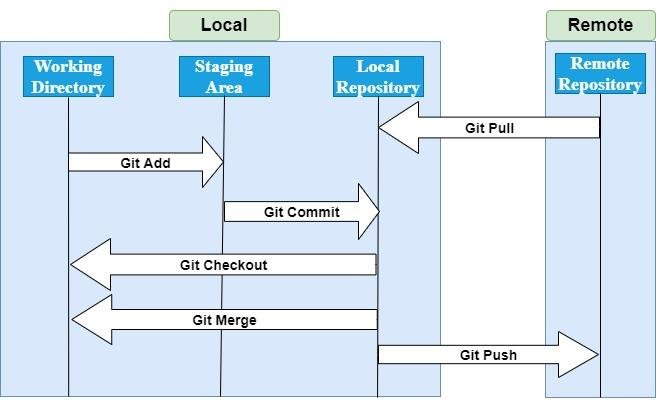
\includegraphics[width=0.6\textwidth]{git_workflow.jpg}
    \caption{workflow}
    \label{fig:Figure 1}
\end{figure}

\section{Version Control of LaTeX Documents}
Using LaTeX with Git involves managing commits effectively. Here is an example of a calculation:
\begin{equation}
    \text{Total Commits} = \text{Branches} \times \text{Commits Per Branch}
\end{equation}
This formula helps estimate the number of commits made across all branches in a repository.



%table
\section{Table in LaTeX}
\begin{table}[h]
\centering
\begin{tabular}{|l|l|l|}
\hline
\textbf{Command}   & \textbf{Purpose}                                  & \textbf{Example}       \\ \hline
git init           & Initialize a new Git repository                  & \texttt{git init}      \\ \hline
git add            & Add files to the staging area                    & \texttt{git add file.txt} \\ \hline
git commit         & Commit changes with a message                    & \texttt{git commit -m "Initial commit"} \\ \hline
git status         & Show the status of the working directory and staging area & \texttt{git status}    \\ \hline
git log            & Show the commit history                          & \texttt{git log}       \\ \hline
\end{tabular}
\caption{Git Commands and Their Usage}
\label{tab:git-commands}
\end{table}
\end{document}
